\documentclass[preprint, 12pt]{elsarticle}

%% Use the option review to obtain double line spacing
%% \documentclass[preprint,review,12pt]{elsarticle}

%% Use the options 1p,twocolumn; 3p; 3p,twocolumn; 5p; or 5p,twocolumn
%% for a journal layout:
%% \documentclass[final,1p,times]{elsarticle}
%% \documentclass[final,1p,times,twocolumn]{elsarticle}
%% \documentclass[final,3p,times]{elsarticle}
%% \documentclass[final,3p,times,twocolumn]{elsarticle}
%% \documentclass[final,5p,times]{elsarticle}
%% \documentclass[final,5p,times,twocolumn]{elsarticle}

%% The graphicx package provides the includegraphics command.
\usepackage{graphicx}
\usepackage{subcaption}
%% The amssymb package provides various useful mathematical symbols
\usepackage{amssymb}
\usepackage{siunitx}
%%\usepackage{authblk}
%% The amsthm package provides extended theorem environments
%% \usepackage{amsthm}

%% The lineno packages adds line numbers. Start line numbering with
%% \begin{linenumbers}, end it with \end{linenumbers}. Or switch it on
%% for the whole article with \linenumbers after \end{frontmatter}.
%% \usepackage{lineno}

%% natbib.sty is loaded by default. However, natbib options can be
%% provided with \biboptions{...} command. Following options are
%% valid:

%%   round  -  round parentheses are used (default)
%%   square -  square brackets are used   [option]
%%   curly  -  curly braces are used      {option}
%%   angle  -  angle brackets are used    <option>
%%   semicolon  -  multiple citations separated by semi-colon
%%   colon  - same as semicolon, an earlier confusion
%%   comma  -  separated by comma
%%   numbers-  selects numerical citations
%%   super  -  numerical citations as superscripts
%%   sort   -  sorts multiple citations according to order in ref. list
%%   sort&compress   -  like sort, but also compresses numerical citations
%%   compress - compresses without sorting
%%
%% \biboptions{comma,round}

% \biboptions{}

\journal{Journal Name}

\begin{document}

\begin{frontmatter}

%% Title, authors and addresses

%\title{Particle--in--cell simulation of the dynamics of short--pulse laser
%irradiated multilayer targets and x--ray reflectometry diagnostics.}

\title{Theoretical study on grazing-incidence x-ray scattering of  surfaces upon high-intensity laser irradiation}


%% use the tnoteref command within \title for footnotes;
%% use the tnotetext command for the associated footnote;
%% use the fnref command within \author or \address for footnotes;
%% use the fntext command for the associated footnote;
%% use the corref command within \author for corresponding author footnotes;
%% use the cortext command for the associated footnote;
%% use the ead command for the email address,
%% and the form \ead[url] for the home page:
%%
%% \title{Title\tnoteref{label1}}
%% \tnotetext[label1]{}
%% \author{Name\corref{cor1}\fnref{label2}}
%% \ead{email address}
%% \ead[url]{home page}
%% \fntext[label2]{}
%% \cortext[cor1]{}
%% \address{Address\fnref{label3}}
%% \fntext[label3]{}


%% use optional labels to link authors explicitly to addresses:
%% \author[label1,label2]{<author name>}
%% \address[label1]{<address>}
%% \address[label2]{<address>}

\author[1]{M. Banjafar}
\author[2]{L. Randolph}
\author[3]{T. Kluge}
\author[3]{M. Bussmann}
\author[1]{A. Mancuso}
\author[3]{T. E. Cowan}
\author[1]{C. Fortmann-Grote}
\author[2]{C. Gutt}
\author[1]{M. Nakatsutsumi}

%%\affil[1]{European XFEL GmbH, }

\address[1]{European XFEL GmbH, Holzkopple 4, 22869 Schenefeld, Germany}
\address[2]{Department of Physics, University of Siegen, D-57072 Siegen, Germany}
\address[3]{Helmholtz-Zentrum Dresden-Rossendorf, Bautzner Landstraße 400, 01328 Dresden, Germany}

\begin{abstract}
%% Text of abstract
  Interaction of solid materials with laser pulses of \SI{1e16}{\watt\per\cm}
  produces warm dense matter under controlled laboratory conditions.
  Multilayer targets of alternating high and low Z material layers of a few
  nanometer thickness open the possibility
  to study the laser--matter interaction dynamics as a volumetric effect by
  observing the multilayer Bragg peak in a x--ray reflectometry experiment.
  Here, we present particle--in--cell simulations of
  the laser and multilayer target interaction and subsequent calculations of
  the reflectivity as a
  function of reflection angle and various time delays between the optical pump
  and the x--ray probe pulse delivered by an x--ray free--electron laser.
  Using the same methodology, we also calculate the diffuse x--ray scattering
  signal.
  We demonstrate that the combined measurement of reflectivity and
  diffuse scattering provides valuable information about the evolution of
  electron density gradients, temperature and ionization as a function of target
  depth and pump--probe time delay and Bragg peak position.
\end{abstract}

\begin{keyword}
Science \sep Publication \sep Complicated
%% keywords here, in the form: keyword \sep keyword

%% MSC codes here, in the form: \MSC code \sep code
%% or \MSC[2008] code \sep code (2000 is the default)

\end{keyword}

\end{frontmatter}

%%
%% Start line numbering here if you want
%%
%%\linenumbers
\begin{verbatim}
Carsten:
* Abstract to be iterated when rest of the text comes into shape.}
* What figures will go in the paper?
Thomas:
  * Experimental description should focus on giving the physical
  motivation of why we want to do surface diffraction at all
  * Simulation part should focus on showing
    (1) the qualitative plasma physics we expect
    (2) the differences between codes with respect to
      (a) different physics included (e.g. comparing with and without
      ionization, with and withou collisions etc)
      (b) different models, e.g.
        i) TF vs. Direct impact ionization
        ii) large collision frequency vs. low collision frequency
        iii) comparing a constant Coulomb logarithm vs. a T-dependent one
        iV) hydro vs. PIC
      (c) different model implementations (e.g. TF and ADK are different
      in PICLS and PIConGPU)
    (3) lay the foundation in showing what plasma physics is important and
    what the uncertainties in the numerical modeling are, so that in the
    scattering part one can focus on showing how to measure the physics
    and validate the codes
  * The scattering part has to derive much more stringent the connection
  between the measured quantities (e.g. beta, change of max(Q) position,
  fourier transform/rings) and plasma physical quantities (e.g. what
  exactly are slow/fast dynamics and how do they imprint on the speckle
  contrast? surface ripple correlation changes - where do they come from
  (should be explained in the sim-part) and how do the show up in the
  signal, what exactly expands and how/why does it imprint on the signal,
  what is the plasma physics measured by the ring-analysis?...)
\end{verbatim}
\begin{verbatim}
TODOS:
  * Add authors, keywords
  * Abstract
  * Find out how many pages we have for the RPHDM proceedings? Depending on this
  info, structure the paper, suggestions below
  * Introduction:
    -Motivation
    - Intensity regime -> WDM, some words about prepulse in high-power laser
    experiments
  * Schematic experiment setup (use figure from talk)
  * Methods:
    - PIC: which code(s), only short, give references. briefly discuss
  collisional ionization and collisions.
    - reflectometry calculations from PIC results
  * Results:
    - electron density plots, maybe video for supplemental material (only Ta-Al,
    or also Ta-Si?)
    - electron density profiles, difference betwen codes (do we want to show
    here, is it checked?)
    - reflection curves, diffuse scattering (?)
  * Discussion
  * Summary, Outlook
\end{verbatim}

%% main text
\section{Introduction}
\label{S:1}

%% motoaki
(1) High-intensity laser-matter (solid) interaction opens broad applications such as ... bra bra ...
(2) Laser-matter coupling is largely dominated by instantaneous electron density 

%%



The warm dense matter regime is a state of matter in which the materials have been exposed to the high pressure of 1 Mbar and have the properties of both plasma and solid state. In such a condition the temperature of the electrons varies from a few eV to 100 eV and the density is typically from solids up to highly compressed. These unique physical properties of WDM and its importance and practical applications in physics of planetary formation like the interior layers structure, convection, magnetic field, and charge transfer inside the gas giants and the core of Earth-like planets [], inertial confinement fusion where the material is encountered during the implosion phase [], plasma optics [], and material science [] have made it an exciting topic to study. However, this unique position of WDM in density and temperature space makes this area of physics very challenging to investigate. Actually, this state of matter can be produced in the laboratory by irradiating a very thin foil with a few tens of nm thickness by femtosecond optical laser pulses with $10^{15}-10^{16}$ $W/cm^2$ intensity []. But, for usual optical diagnostic techniques, WDM acts like an opaque because of the high density of free electrons. Thus, in order to obtain physical information like density profile and temperature from inside the WDM other techniques such and proton and X-ray radiography have been commonly using [].

Some novel techniques in laser--plasma interactions such and plasma mirrors[], in which a femtosecond laser pulse is efficiently reflected by the dense plasma with higher temporal contrast and tighter focusing, and using pre-pulses [], which often precede the main high-intensity laser pulse, are categorized in the WDM regime due to the up to $10^{16}$ $W/cm^2$ intensity of the laser pulses that is commonly used in these technique. In these cases, having a good knowledge of the surface structure such as nano-scale roughness and surface dynamics like plasma hydrodynamic expansion is very important to optimize the experiments. Here, X-ray free electron laser (XFEL) has the capability to provide high temporal (femtosecond) and spacial (nanometer) resolution that is crucial to get some information from the surface of hot dense plasma. It also provides a very good vision of electron density gradient and the opacity [] of warm dense plasma. Some X-ray probing techniques such as X-ray reflectivity (XRR) and grazing incidence X-ray diffraction (GIXD) [] are particularly sensitive to the sample electron distribution in the plane and in the direction perpendicular to the substrate surface, by which we are able to simply obtain the depth-resolved structure characterization by altering the incidence angle.

In this work, we present Particle--in--Cell simulation and X--ray reflectometry study of interaction of a $10^{16}$ $W/cm^2$ intensity optical laser pulse with a multilayer target based on an experiment with the same geometry.

\section{Experiments}

A brief explanation about the theory.

\section{Modeling}
\label{S:2}
\subsection{Particle--in--Cell simulation}
A schematic of 2D PIC simulation setup has been shown in (figure). The simulation was done by PIConGPU code [reference] on $4096 \times 4096$ cells that the dimension of each cells is 2.5 {\AA} in both direction and the time step is ${\Delta}t=5.89 \times 10^{-4}$ fs. Thus, the dimension of simulation box is nearly $1 \times 1$ $\mu m$ and the total time of simulation is 527 fs. An optical laser pulse with plane wave profile, intensity $I = 10^{16}$ $W/{cm}^2$ corresponds to $a_{0} = 0.068$ for 800 $nm$ laser wavelength, and the pulse duration $\tau_{FWHM}=50$ fs, and focal spot size of 5 $\mu m$  comes alongside the $y$ axis and incidents normally on the front of multilayer (ML) target, which is a 10 times reps of Tantalum, $n_{Ta} = 5.55 \times 10^{22}$ $cm^{-3}$, and Aluminum ,$n_{Al} = 6.022 \times 10^{22}$ $cm^{-3}$, double-layers. The thickness of each layer is 5 $nm$ and regarding the 20 $nm$ Silicon substrate, the total thickness of the target is 120 $nm$. Three kinds of ionization model, barrier suppression ionization (BSI) [reference], Thomas-Fermi (TF) [reference], and the tunnel ionization (ADK) [reference] have been used in our simulation, while it dose not include the collision process. In fact, quantitative modeling of WDM is a critical challenge for kinetic method such as particle--in--cell and radiation--hydrodynamics mainly due to (a) difficulties in describing the ionization dynamics; (b) uncertainty about electron-ion collision frequency which governs absorption, heat transfer and plasma conductivity; and (c) violation of the heat conduction models at the steeped temperature gradient present in laser excited plasma []. However,

\begin{figure}[h]
\centering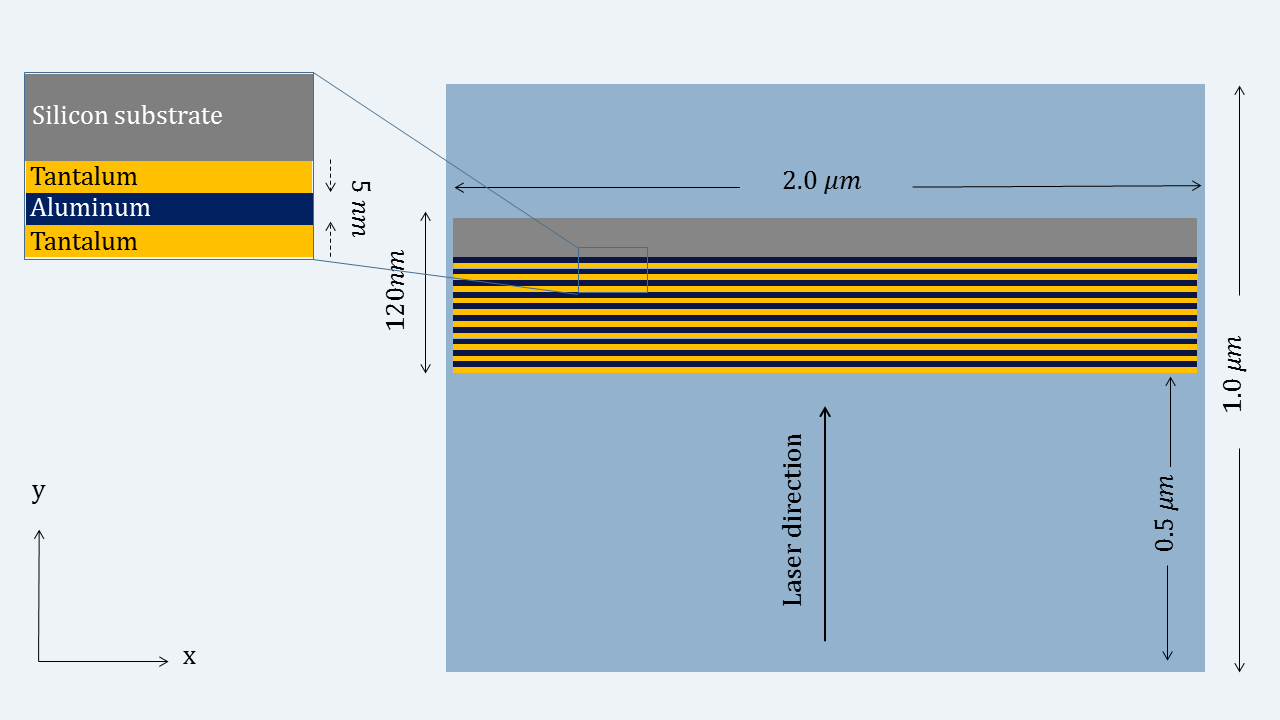
\includegraphics[width=0.8\linewidth]{P_2.png}
\caption{A schematic of PIC simulation setup}
\end{figure}

\subsection{X-ray diffraction}

\section{Results and discussion}
The figure (figure) is a closeup view the free (first row), bound (second row), and total electron density (third row) 2D maps at 0, 75, 226, and 410 fs of the PIC simulation. The maximum intensity of the lase pulse reaches the target at the time 0 and it goes of the simulation box around 75 fs. One can easily see the ionization process and generation of free electrons, reduction of bound electrons, and the evolution of total electron density when the laser pulse irradiates the target and even after that. Due to skin depth of Ta and Al the laser pulse is not able to penetrate more than a few nanometer into the target and will be partially reflected when it reaches the critical density, but due to the laser ponderomotive force electrons at the front of target will be pushed into the deeper layers. Regarding the high density of target, which is hundreds of the critical density, and the intensity of laser the term of $\vec{J} \times \vec{B}$ acceleration is negligible compare the dc-ponderomotive [reference]. However, due to penetration of laser into the skin depth, the magnetic part of Lorentz force is able to drag some electrons and pull them out into the vacuum causing the field is maintained zero inside the target [reference]. The most of the dragged electrons will be pushed back into the target by inversing the laser field during a cycle causing an oscillation perpendicular to the surface of the target.

By following up the total electron density evolution in figure (figure), one can easily see that the surface of the layers get more roughed and those roughness become lager by the time. It also can be seen in figure (diffraction images), which displays three diffraction pattern as a function of $Q$ in x and y direction in ln-scale corresponding to -51.8, 160.3, and 341.9 fs. The diffraction images show the specular signal as a high intensive streak and also the diffuse scattering signal as a ring around the center by which we are able to interpret the scale of the roughness. That means larger ring for diffuse scattering signal corresponds to the smaller scale roughness and vice versa. By this definition, we can relate the large ring at -51.8 fs to the angstrom scale roughness which are mainly due to random distribution of particles inside the angstrom scale simulation cells. By the time the ring gets smaller and for larger $Q$-values there is only a weak scattering signal that means the scale of the roughness gets lager due to the irradiation. This dynamic can also be seen in figure (radial intensity figure a) shows a more detailed distribution of the radial intensity of scattered X-ray as a function of $Q$ for different time from -70 fs (red) to 395.9 fs (blue). Figure (radial intensity figure a) depicts the maximum of the scattered intensity as a function of time displaying a reduction of intensity until its minimum value at 124.6 fs that correspond to the three quarter of optical laser pulse.

\begin{figure}[h]
\centering
\includegraphics[width=1.0\linewidth]{paper_plot.png}
\caption{2D electron density maps}
\end{figure}

The figure (figure) shows the averaged total electron density along the transverse direction in which 0 fs shows the moment that peak of the laser pulse reaches the surface of the target and 75.4 fs is right after the laser pulse. It can obviously be seen that due to the radiation pressure during the laser pulse, almost there is no expansion on the surface of the target. Besides that, the ML target maintains its structure without significant change. After the laser pulse at 75.4 fs see a few nanometer expansion of the electrons but latter due to the hydrodynamic expansion, the surface expands rapidly up to 20 $nm$  until 226 fs, and then with a lower speed up to 40 $nm$ until 452 fs. At the same time, the ML structure is deformed by the distribution of the free electrons throughout the target. This dynamic of electron density can also be seen in figure (contrast figure) that shows the scattered X-ray intensity fluctuations by speckle contrast $\beta$. As we mentioned earlier, the higher value of $\beta$ corresponds slower dynamics and it happens at the maximum intensity of the laser pulse at 0 fs. Then, $\beta$ curve drops down rapidly that corresponds to smaller intensity fluctuations and faster dynamics until 226 fs, from then it the dynamics get faster with a slower speed. It is also shown in figure (Q as time figure) that displays the variation of the Q-value as a function of time for the maximum scattered X-ray intensity. Similar to the figure (contrast figure), at 75.4 fs, right after the optical laser pulse, the Q-value drops down to the 0.5 $nm^{-1}$ which means the scale of the roughness get larger during this time. One can interpret the speed of the expansion from the slope of this graph. For instance, from 75.4 to 200 fs, Q changes by 2 $nm^{-1}$ that corresponds $\approx 1.5$ $nm$ in real space. Thus, the speed of the plasma expansion during this time is about $10^{4}$ $m/s$.

\begin{figure}[h]
\centering
\includegraphics[width=0.8\linewidth]{Paper_plot_1D.png}
\caption{1D total electron density maps}
\end{figure}

To have a better image of these dynamics we considered some $Q$-rings with the width of $\Delta Q \approx 0.08$ $nm^{-1}$ and different radius from 0.54 to 7.60 $nm^{-1}$ which are centered at the center of diffraction pattern ring as it has been shown in figure (figure 5a of Lisa). The radius difference between the rings is $\Delta Q_r \approx 0.08$ $nm^{-1}$. Figure (5b from Lisa) shows the variation of the contrast $\beta$ for the smaller $Q$-rings up to radius 3.06 $nm^{-1}$ and figure (5c from Lisa) shows larger $Q$-rings. For the smaller $Q$-rings which correspond to lagers scale roughness we see just a small variation of contrast $\beta$. For instance, for 0.54 and 1.04 $nm^{-1}$, corresponds to (length scale! ask Lisa) $nm$ in real space, one can just see some fluctuations for $\beta$ by the time that means in large scale we are not significant dynamics. But as we go to the larger $Q$-ring values there is an obvious reduction of $\beta$ and faster dynamics for smaller scale roughness.

\section{Conclusion}

a short conclusion.

\section{Acknowledgment}
text
\newline
\newline
\newline
\newline
\newline


To add the equations, tables, plots, and bullet points use these items:

\begin{equation}
\label{eq:emc}
e = mc^2
\end{equation}

\begin{figure}[h]
\centering
\includegraphics[width=0.4\linewidth]{placeholder}
\caption{Figure caption}
\end{figure}

\begin{table}[h]
\centering
\begin{tabular}{l l l}
\hline
\textbf{Treatments} & \textbf{Response 1} & \textbf{Response 2}\\
\hline
Treatment 1 & 0.0003262 & 0.562 \\
Treatment 2 & 0.0015681 & 0.910 \\
Treatment 3 & 0.0009271 & 0.296 \\
\hline
\end{tabular}
\caption{Table caption}
\end{table}

\begin{itemize}
\item Bullet point one
\item Bullet point two
\end{itemize}

\begin{enumerate}
\item Numbered list item one
\item Numbered list item two
\end{enumerate}

%% The Appendices part is started with the command \appendix;
%% appendix sections are then done as normal sections
%% \appendix

%% \section{}
%% \label{}

%% References
%%
%% Following citation commands can be used in the body text:
%% Usage of \cite is as follows:
%%   \cite{key}          ==>>  [#]
%%   \cite[chap. 2]{key} ==>>  [#, chap. 2]
%%   \citet{key}         ==>>  Author [#]

%% References with bibTeX database:

\bibliographystyle{model1-num-names}
\bibliography{sample.bib}

%% Authors are advised to submit their bibtex database files. They are
%% requested to list a bibtex style file in the manuscript if they do
%% not want to use model1-num-names.bst.

%% References without bibTeX database:

% \begin{thebibliography}{00}

%% \bibitem must have the following form:
%%   \bibitem{key}...
%%

% \bibitem{}

% \end{thebibliography}


\end{document}

%%
%% End of file `elsarticle-template-1-num.tex'.
